\documentclass[12pt]{amsart}
\usepackage{tikz}
\usetikzlibrary{arrows, matrix, positioning,fit}

\tikzset{
    % Good spacing hack (the ghost mode)
     gs/.style={
        rectangle,
        thick,
        text width=3em,
        align=center,
        draw=white,
        rounded corners,
        minimum height=2em
    },    %
    rc/.style={rectangle,
        thick,rounded corners,draw},
    lfe/.style={rc,
        text width=12em,
        align=center,
        text=magenta
    },
    % Long focus effect bis
    lfeb/.style={rc,
        text width=12em,
        align=center,
        text=violet
    },
}


\begin{document}

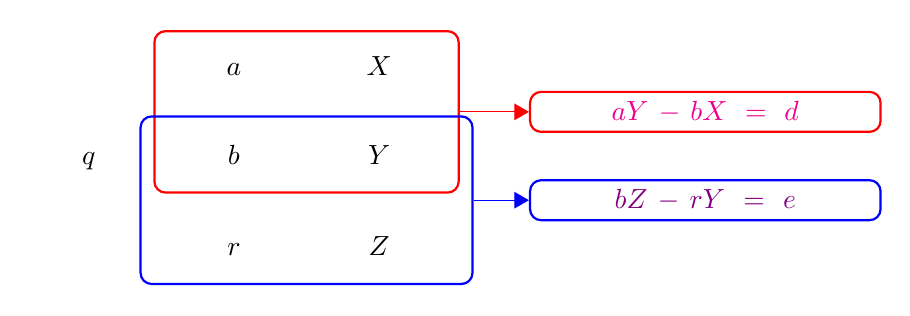
\begin{tikzpicture}
    \matrix[matrix of nodes,nodes=gs,
        row sep    = 1em,
        column sep = 1.5em,
    ](mat){
          & $a$ & $X$ \\
$q$ & $b$ & $Y$  \\
          & $r$ & $Z$  \\
    };

    \node[fit=(mat-1-2) (mat-2-3),inner xsep=1em,rc,red] (F1){};

    \draw[red,-triangle 60] (F1.east) -- ++ (2.5em,0)
               node[right, lfe] (f){$aY - bX = d$};

    \node[inner xsep=1.5em,fit=(mat-2-2) (mat-3-3),rc,blue] (F2){};

    \draw[blue,-triangle 60] (F2.east) -- ++ (2em,0)
               node[right,lfeb] (f){$bZ - rY = e$};
\end{tikzpicture}

\end{document}